%\usepackage{tikz}
%\usetikzlibrary{arrows.meta}
%\begin{document}
\begin{center}
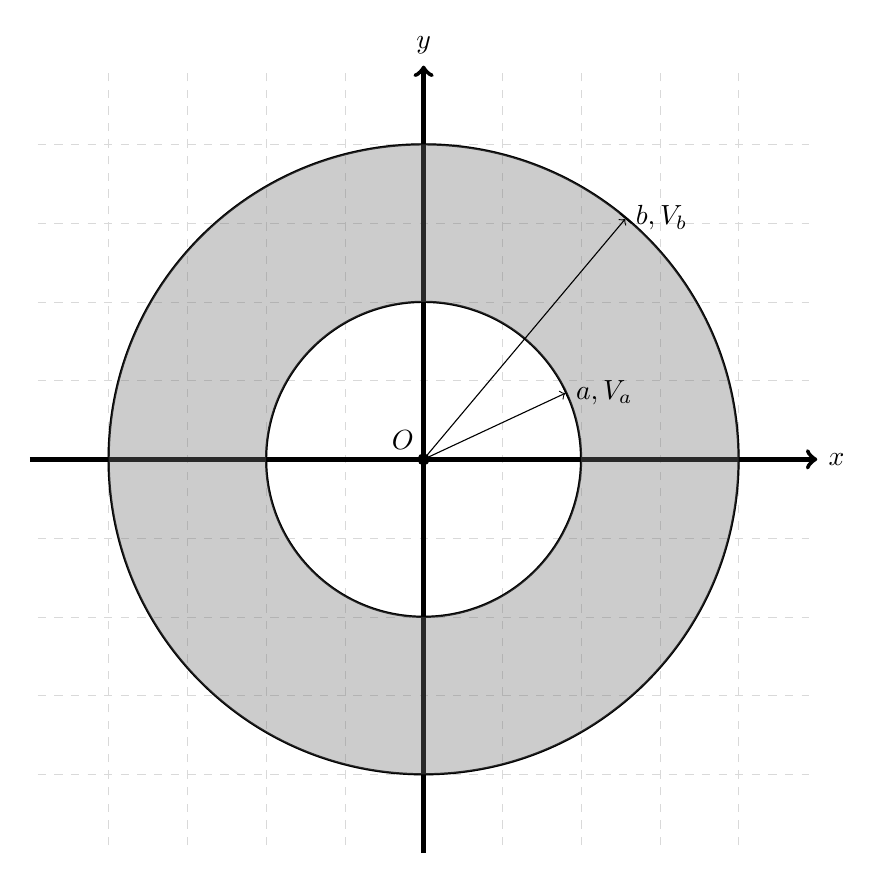
\begin{tikzpicture}

\draw[help lines, color=gray!30, dashed] (-4.9,-4.9) grid (4.9,4.9);
\draw[->,ultra thick] (-5,0)--(5,0) node[right]{$x$};
\draw[->,ultra thick] (0,-5)--(0,5) node[above]{$y$};

\draw [thick] circle [radius=2];
\draw [thick] circle [radius=4];

\draw[double = gray!40, double distance=2cm, opacity=0.2] (0,0) circle (3);

\draw[->|, rotate around={25:(0,0)}] (0,0) -- (2,0)  node [right] {$a,V_a$};
\draw[->|, rotate around={50:(0,0)}] (0,0) -- (4,0)  node [right] {$b,V_b$};
\draw[fill=black](0,0) circle (2 pt) node [anchor=south east] {$O$};

\end{tikzpicture}
\end{center}